% figure.tex
\documentclass[tikz, border=15pt]{standalone}
\usepackage{xeCJK}
\usepackage{tikz}
% 英文字体设置
\setmainfont{Alegreya}
\setsansfont{Alegreya}

% 中文字体设置
\setCJKmainfont{仓耳今楷04 W04}
\setCJKsansfont{仓耳今楷04 W04}

\usetikzlibrary{arrows.meta, shapes, positioning, calc, fit}

\begin{document}
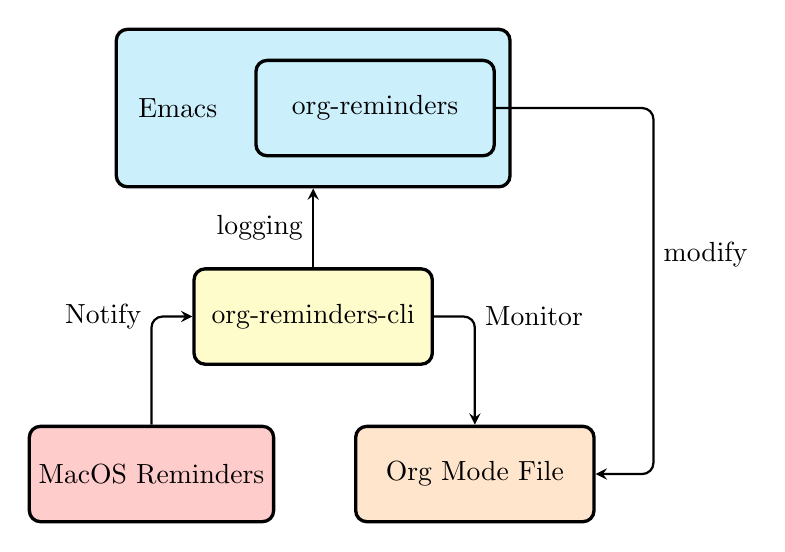
\begin{tikzpicture} [
    module/.style={draw, very thick, rounded corners, minimum
    width=20ex, minimum height=8ex, align=center},
    red-module/.style={module, fill=red!20},
    orange-module/.style={module, fill=orange!20},
    yellow-module/.style={module, fill=yellow!20},
    cyan-module/.style={module, fill=cyan!20},
    arrow/.style={-stealth, thick, rounded corners},
  ]

  \newcommand{\splitarrow}[3]{
    \path (#1) -- (#2) node[midway] (tmp) {#3};
    \draw[thick, rounded corners] (#1) -- (tmp);
    \draw[arrow] (tmp) -- (#2);
  }

  \node[red-module] (reminders) {MacOS Reminders};
  \node[orange-module, right=of reminders] (org-mode) {Org Mode File};
  \node[yellow-module] (org-reminders-cli) at ($
  (reminders)!0.5!(org-mode) + (0, 2) $)
  {org-reminders-cli};
  \node[cyan-module, above=of org-reminders-cli,
    minimum width = 5cm,
    minimum height = 2cm,
    label={[anchor=west, xshift=5pt]west:Emacs}
  ] (emacs) {};
  \node[module, anchor=east, xshift=-2mm] (org-reminders) at
  (emacs.east) {org-reminders};

  \draw[arrow] (reminders) |- (org-reminders-cli) node[left, midway] {Notify};
  \draw[arrow] (org-reminders-cli) -| (org-mode) node[right, midway] {Monitor};
  \draw[arrow] (org-reminders-cli) -- (emacs) node[midway, left] {logging};
  \draw[arrow] (org-reminders.east) -- ++(2cm,0)|- (org-mode.east) node[pos=0.2,
  right] {modify};

\end{tikzpicture}
\end{document}
